\documentclass[fontsize=11pt]{scrartcl}
%-------------------------------------------------------------------------------------------------
% LATEX TEMPLATE FOR A BACHELOR'S THESIS AT GHENT UNIVERSITY GLOBAL CAMPUS
% CREATED BY MANVEL GASPARYAN
% APRIL, 2021
%-------------------------------------------------------------------------------------------------
\usepackage{hyperref, tikz, float, subfigure, multicol, amsmath, amsthm, alphalph, amsfonts, amssymb, geometry, enumitem, parskip, xcolor, sectsty}
\usepackage[normalem]{ulem}
\usepackage[font=scriptsize,labelfont=bf]{caption}
\usepackage[explicit]{titlesec}
\usepackage[scaled]{helvet}
\renewcommand\familydefault{\sfdefault} 
\usepackage[T1]{fontenc}

\usepackage{setspace}

\usepackage{{listings}}

%-------------------------------------------------------------------------------------------------
 \geometry{a4paper, total={170mm,257mm}, left=20mm, right=20mm, top=25mm, bottom=30mm}
%-------------------------------------------------------------------------------------------------
\newtheorem{proposition}{Proposition}[section]
\newtheorem{lemma}{Lemma}[section]
\newtheorem{remark}{Remark}[section]
\newtheorem{corollary}{Corollary}[section]
\newtheorem{definition}{Definition}[section]
%-------------------------------------------------------------------------------------------------
\pagenumbering{roman}
\usepackage{fancyhdr}
\pagestyle{fancy}
\fancyhf{}
\renewcommand{\headrulewidth}{0pt}
\rhead{}
\lhead{}
\rfoot{\thepage}
\lfoot{}

%-------------------------------------------------------------------------------------------------
\definecolor{ghent_blue}{rgb}{0.1176, 0.392, 0.7843}
\definecolor{ghent_dark}{rgb}{0.0, 0.2, 0.4}
%-------------------------------------------------------------------------------------------------
\title{{\color{ghent_blue} TITLE: LATEX TEMPLATE FOR A BACHELOR'S THESIS AT GHENT UNIVERSITY GLOBAL CAMPUS}}
\subtitle{{\color{ghent_dark} [DOCUMENT SUBTITLE]}}
\date{}         
%-------------------------------------------------------------------------------------------------
\sectionfont{\fontsize{16}{15}\selectfont}
\sectionfont{\color{ghent_blue}}
%=================================================================================================
\begin{document}
%=================================================================================================
%PAGE i: TITLE PAGE 1
%-------------------------------------------------------------------------------------------------
\thispagestyle{empty}
\hfill
\includegraphics[scale = 1]{img/badge/2021.png}\\
%-------------------------------------------------------------------------------------------------
\vspace{8cm}

\noindent{\fontsize{30}{50}\selectfont{\color{ghent_blue}\noindent \hspace{12mm}\textbf{
Microphotonics %TITLE
}}}\\
\fontsize{20}{50}\selectfont{\color{ghent_dark}\noindent \hspace{13mm}\textbf{
CAD-LAB: Periodic Structure%SUBTITLE
}}\vspace{10mm}

\hspace{10mm}{\fontsize{10}{10}\selectfont{\textbf{
Lukuan Zhang, Rui Zhu, Xiyuan Guo%AUTHOR
}}}
\vspace*{\fill}
%-------------------------------------------------------------------------------------------------
\begin{flushleft}
\begin{figure}[b!]

\includegraphics[scale = 1.4]{img/badge/GUGC.pdf}
\end{figure}
\end{flushleft}

\doublespacing
\tableofcontents
\pagebreak
\pagenumbering{arabic}
%=================================================================================================
%HELP
%-------------------------------------------------------------------------------------------------
\section*{*  \uline{HELP}}
Once have been refered you can delete this part.\\
If you want to write an inline equation, code like this $E=mc^2$.\\
If you want to write a displayed equation without numbering, code like this $$E=mc^2$$\\
If you want to write a numbering displayed equation, code like this
\begin{equation} 
    E=mc^2 \label{eq1}
\end{equation}
and you can quote the equation by using Eq.\ref {eq1}.\\
\textbf{Tips:} The software \verb|Mathpix| can convert images and PDFs to LaTeX format which is
highly recommended by me.\\
List items like this:
\begin{enumerate} % itemize/description
    \item contents
    \item contents
\end{enumerate}
If you want to add one or more images as Figure \ref{name1} shown, you can copy the
code as following.\\
\begin{figure}[H]
    \centering
     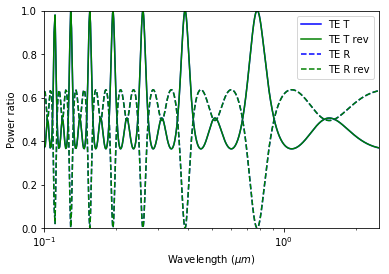
\includegraphics[width=0.35\textwidth]{img/1.png} % set width to get a proper ratio
     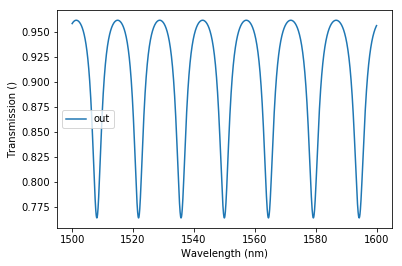
\includegraphics[width=0.35\textwidth]{img/2.png}
     \caption{Here to write the caption of the figure.}
     \label{name1}
\end{figure}
{\color{ghent_blue}Some details to notice:}
\begin{enumerate}
    \item  \textbf{Function name} and \textbf{units} should be presented in the Roman Regular Font.
    We can do this by using the sign backslash such as $\log(x)$, $\sin(x)$, $\cos(x)$, etc.
    \item When writing source codes in \LaTeX, make sure that the one-line code length 
    \textbf{does not} exceed one page(or 1/2 screen width on computer). Too long in width makes 
    a worse reading experience.
    \item Everytime when the new task comes, you are allowed to copy the whole template file and 
    rename it into the task name, then modify on the copy. Please don't modify the code directly
    on the template.
    \item Don't forget enter a space after the punstuation marks.
\end{enumerate}



%=================================================================================================
\pagebreak
%=================================================================================================
%TASK 1
\section{\uline{Distributed Bragg Refector}}
%-------------------------------------------------------------------------------------------------
%-------------------------------------------------------------------------------------------------
% Here comes some text. This text makes use of 1.5 line spacing. 
%-------------------------------------------------------------------------------------------------
\subsection{}
%-------------------------------------------------------------------------------------------------
From Figure \ref{fig1.1} of the $k$-vector diagram of the surface grating, 
the period of surface grating is calculated as $0.917\mathrm{\mu m}$.
\begin{figure}[H]
    \centering
     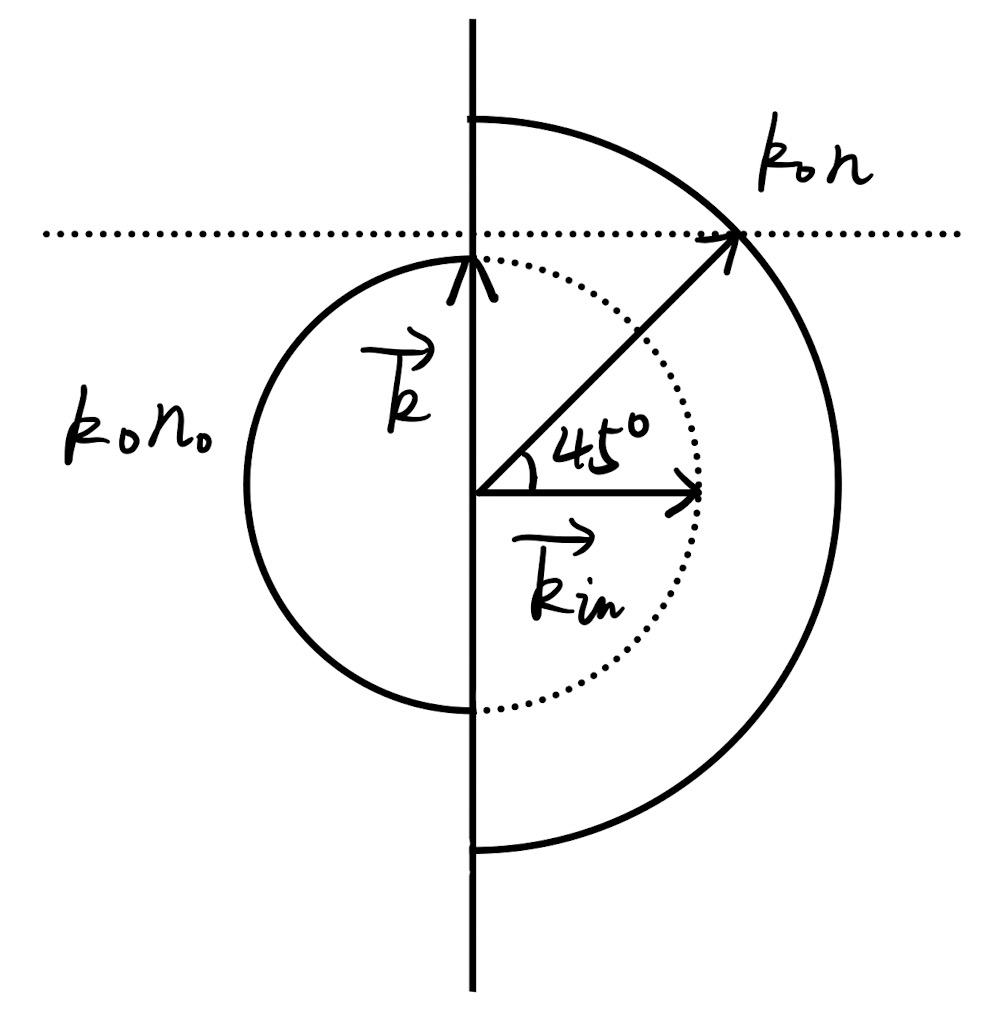
\includegraphics[width=0.4\textwidth]{img/fig1.1.png}
     \caption{The $k$-vector diagram of the surface grating}
     \label{fig1.1}
\end{figure}
%-------------------------------------------------------------------------------------------------
\subsection{}
%-------------------------------------------------------------------------------------------------
Set $D$ as $0.1\mathrm{\mu m}$ and period $\Lambda$ to $0.917\mathrm{\mu m}$ and 
run the simulation, then we can get Figure \ref{fig1.2}, 
which shows the plane wave mainly propagates in the $0^\circ$ direction, 
and partly propagates in the $45^\circ$ and $-45^\circ$ direction.
\begin{figure}[H]
    \centering
     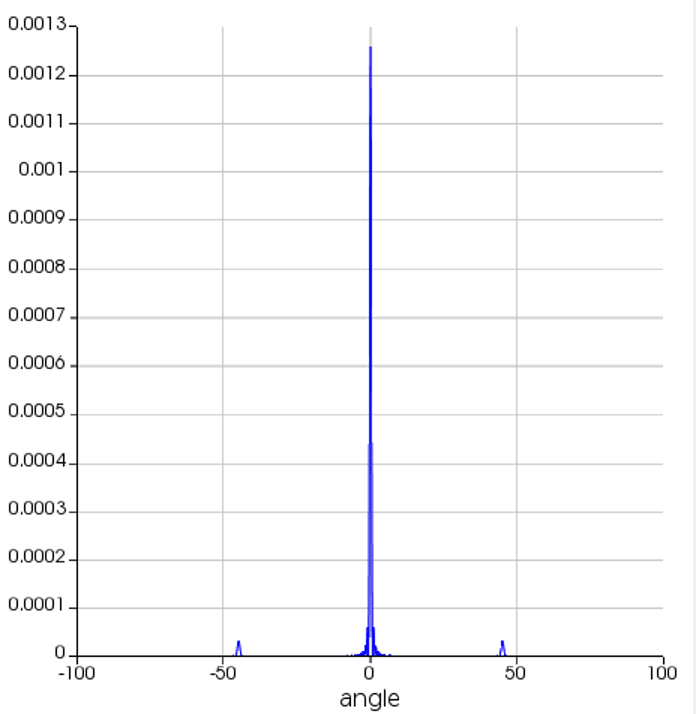
\includegraphics[width=0.45\textwidth]{img/fig1.2.png}
     \caption{Distribution of E2 in farfield with 
     period $0.917\mathrm{\mu m}$ and $D$ $0.1\mathrm{\mu m}$}
     \label{fig1.2}
\end{figure}
%-------------------------------------------------------------------------------------------------
\subsection{}
%-------------------------------------------------------------------------------------------------
\textbf{1. Increase the diffraction to the $45^\circ$ orders}

From Figure \ref{fig1.3}, an analytical expression can be figured out 
as $k_{0}\left(\sqrt{2} D n-n_{0} D\right)=2 \pi m$. For $\lambda=1.55\mathrm{\mu m}$, 
$n=2.39$, $n_0=1$ and $m=1$, we get $D=0.6513\mathrm{\mu m}$. 
Adjusting the parameters and running the simulation again, 
we can see an apparent improvement in Figure \ref{fig1.4}
\begin{figure}[H]
    \centering
     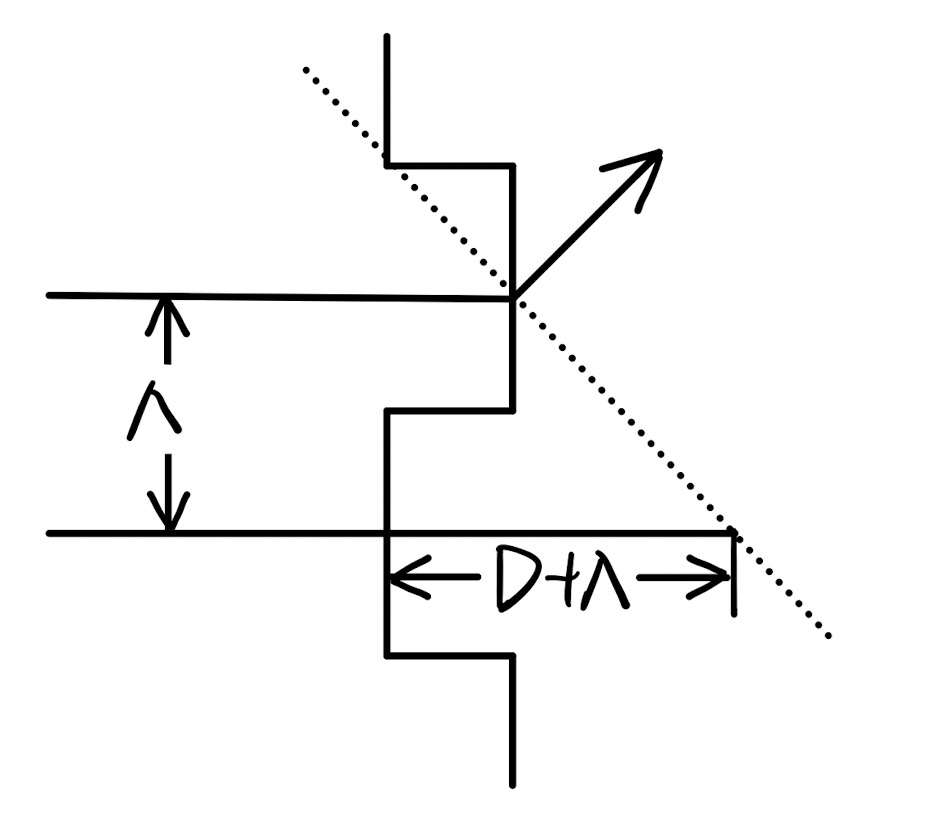
\includegraphics[width=0.4\textwidth]{img/fig1.3.png}
     \caption{The surface gating diagram}
     \label{fig1.3}
\end{figure}
\begin{figure}[H]
    \centering
     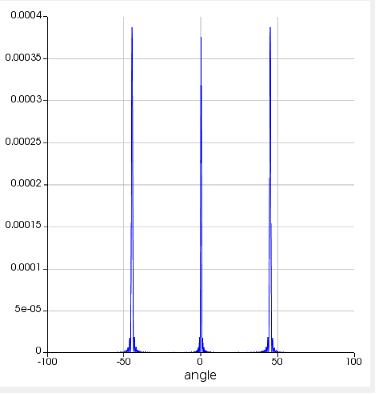
\includegraphics[width=0.45\textwidth]{img/fig1.4.png}
     \caption{Distribution of E2 in farfield with 
     period $0.917\mathrm{\mu m}$ and $D$ $0.6513\mathrm{\mu m}$}
     \label{fig1.4}
\end{figure}

\textbf{2. Decrease the $0^\circ$ diffraction}

From Figure \ref{fig1.3}, an analytical expression can be figured out as
$k_{0}\left((D+\Lambda) n-n_{0} D\right)=2 \pi m$. 
For $\lambda=1.55\mathrm{\mu m}$, $\Lambda=0.917\mathrm{\mu m}$, 
$n=2.39$, $n_0=1$ and $m=1$, we get $D=0.6536\mathrm{\mu m}$. 
Adjusting the parameters and running the simulation again, 
we can also see an apparent improvement in Figure \ref{fig1.6}.
\begin{figure}[H]
    \centering
     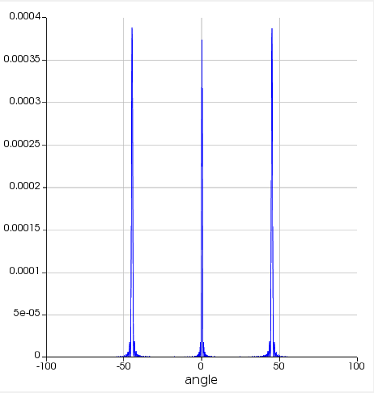
\includegraphics[width=0.45\textwidth]{img/fig1.6.png}
     \caption{Distribution of E2 in farfield with 
     period $0.917\mathrm{\mu m}$ and $D$ $0.6536\mathrm{\mu m}$}
     \label{fig1.6}
\end{figure}


%=================================================================================================
\pagebreak
%=================================================================================================
%TASK 2
%-------------------------------------------------------------------------------------------------
\section{\uline{Surface Grating}}
According to the k-diagram in Figure \ref{k-dia-BR}, we can calculate the period required,
\begin{equation}
    \Lambda=\frac\lambda{2n_{neff}}=0.322917\mu m
\end{equation}
\begin{figure}[H]
    \centering
    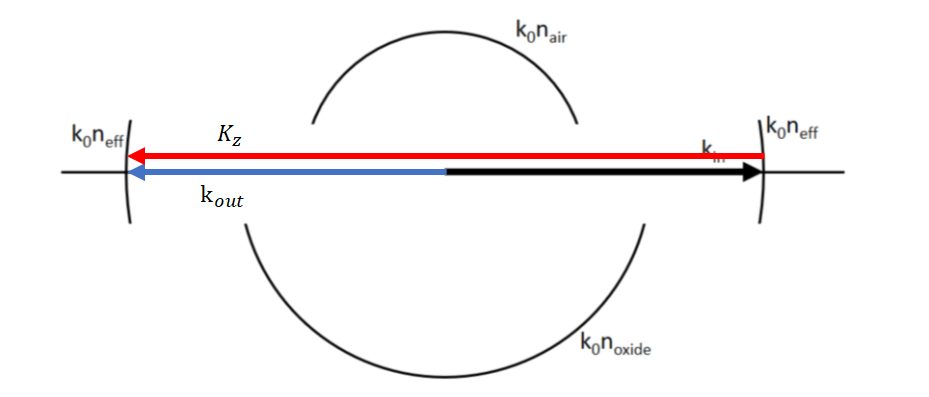
\includegraphics[width=0.7\textwidth]{img/k-dia-BR.png}
    \caption{$\kappa$ vector diagram}
    \label{k-dia-BR}
\end{figure}
\begin{figure}[H]
    \centering
    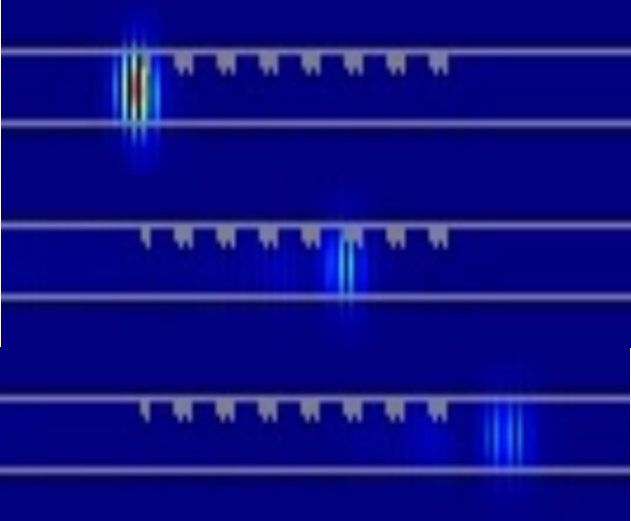
\includegraphics[width=0.4\textwidth]{img/n2.4_mov.png}
    \hspace{10mm}
    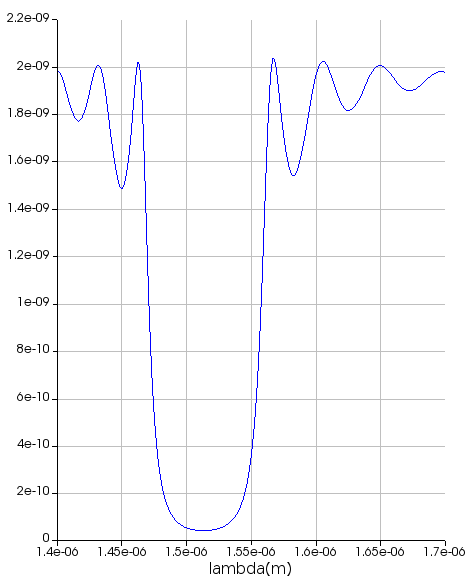
\includegraphics[width=0.4\textwidth]{img/n2.4_T.png}
    \caption{Propagation process(Left). The transmission spectrum of the grating(Right) }
    \label{n2.4_porpa}
\end{figure}
Adjusting it in the \textit{WaveguideGrating.fsp} simulation file,
the result is shown in Figure \ref{n2.4_propa}. Obviously, it is not what we expect.
The smallest transmission is not at $\lambda=1.55\mu m$. We think it's because the air surounding and boundary condition or other
reasons that have influences on the effective refractive index. If the simulation is real,
the real $n_{eff}$ should meet, \\
$$ \frac{\lambda '}{2n_{eff }'}=\frac{\lambda }{2n_{eff }}$$
Then we get $n_{eff}=2.346$ and $\Lambda=0.3304$. In the simulation, we get the reflectivity 0.972.
According to formula $(6.87)$, we calculate $\kappa$,
$$\kappa=\frac 1{2N\Lambda}\ln{\frac{1+\sqrt R}{1-\sqrt R}}=0.250 \mu m^{-1}$$
\begin{figure}[H]
    \centering
    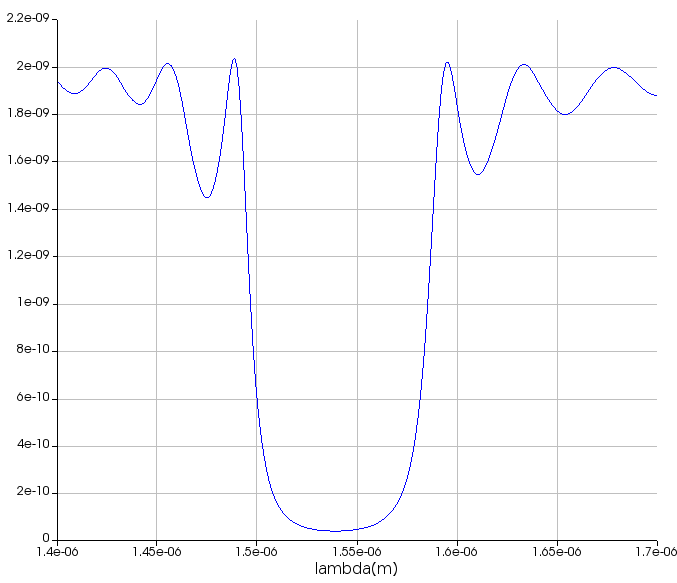
\includegraphics[width=0.4\textwidth]{img/n2.3._Tpng.png}
    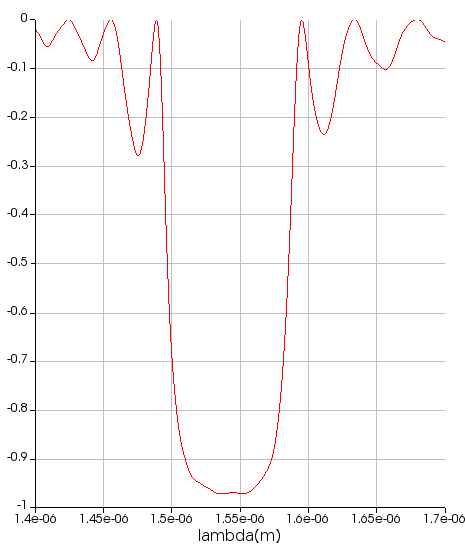
\includegraphics[width=0.4\textwidth]{img/R.png}
    \caption{The transmission spectrum of the grating when $n_{eff}=2.346$(Left). The reflectivity(Right) }
    \label{n2.4_porpa}
\end{figure}
After changing $N$, we could get the relation between $\kappa L$ and $R$, as shown in Figure \ref{Rk}.
Obviously, $L$ is proportional to $\tanh^{-1}{\sqrt R}$. Simulating it with Matlab, we get$\kappa=0.2292\mu m^{-1}$.
\begin{figure}[H]
    \centering
    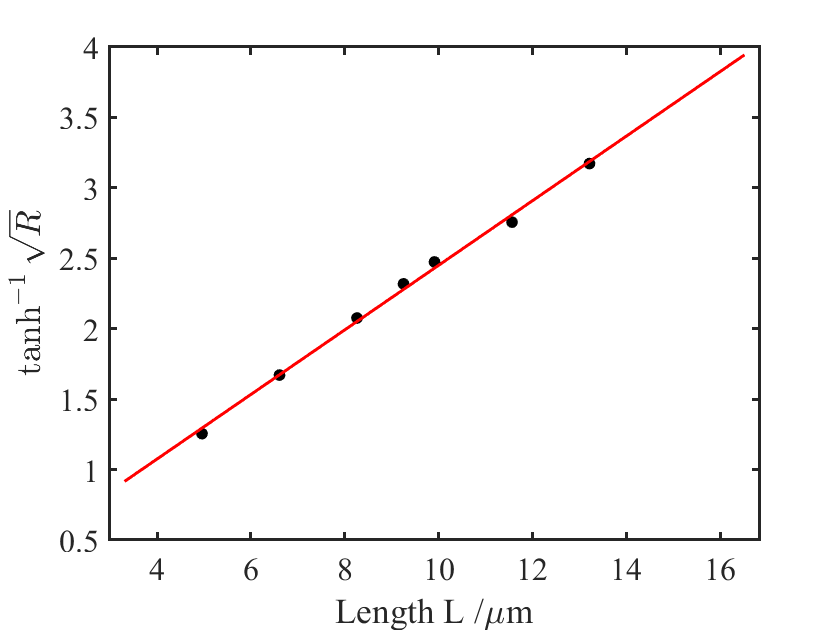
\includegraphics[width=0.7\textwidth]{img/kappa.png}
    \caption{Relation between $\tanh^{-1}{\sqrt R}$ and $L$. }
    \label{Rk}
\end{figure}
\pagebreak
%=================================================================================================
%TASK 3
%-------------------------------------------------------------------------------------------------
\section{\uline{Grating Coupler}}
%-------------------------------------------------------------------------------------------------
% Here comes some text. This text makes use of 1.5 line spacing. 
%-------------------------------------------------------------------------------------------------
\subsection{}
%-------------------------------------------------------------------------------------------------
From Figure \ref{fig3.1.1} of the $k$-vector diagram of the waveguide grating, 
the period of waveguide grating is calculated as $0.645\mathrm{\mu m}$.
\begin{equation}
    K=\frac{2 \pi}{\Lambda}=k_{i n}=\frac{2 \pi}{\lambda} n_{e f f}
\end{equation}
\begin{equation}
    \Lambda=\frac{\lambda}{n_{\text {eff }}}=\frac{1550 \mathrm{~nm}}{2.4}=645.8 \mathrm{~nm}
\end{equation}  
\begin{figure}[H]
    \centering
     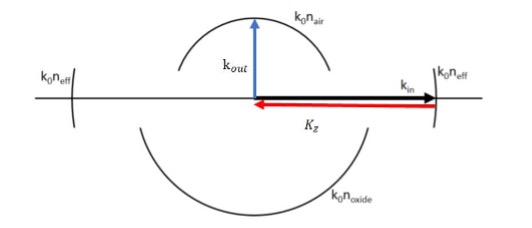
\includegraphics[width=0.7\textwidth]{img/fig3.1.jpg}
     \caption{The $k$-vector diagram of the waveguide grating}
     \label{fig3.1}
\end{figure}
%-------------------------------------------------------------------------------------------------
\subsection{}
%-------------------------------------------------------------------------------------------------
Figure \ref{fig3.2} shows transmission spectrum when the light propagates upwards. 
There is a dip around $1550\mathrm{nm}$, not as expected. 
In theory, there may be a peak instead of a dip at about $1550\mathrm{nm}$. 
The reason is that $n_{eff}$ is smaller than the theoretical value $2.4$ 
for the periodic structure. 
The effective refractive index of unetched part waveguide is 2.4, 
but the etched part is smaller, 
so the effective refractive index of the whole waveguide is smaller than 2.4.
\begin{figure}[H]
    \centering
     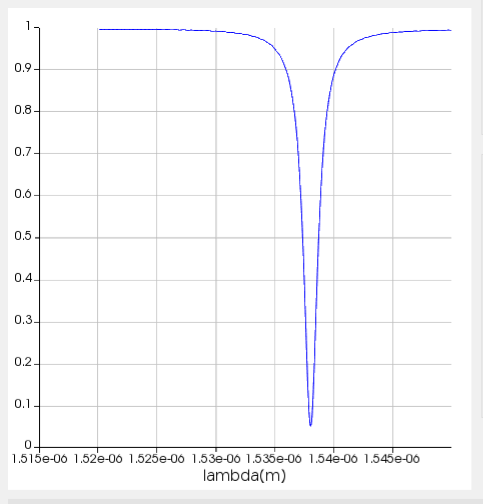
\includegraphics[width=0.45\textwidth]{img/fig3.2.png}
     \caption{Transmission spectrum of monitor\_up at $\Lambda=645.8\mathrm{nm}$}
     \label{fig3.2}
\end{figure}
%-------------------------------------------------------------------------------------------------
\subsection{}
%-------------------------------------------------------------------------------------------------
Figure \ref{fig3.3} shows the far-field radiation pattern of upward. 
The maximum of $E$ is only $1.5\times 10^{-7}$. 
By varying the wavelength, we found that $E$ reach the maximum $7.3\times 10^{-7}$ 
at $\lambda=1468.7\mathrm{nm}$. This wavelength also corresponds to 
the peak of transmission spectrum when the light propagates upwards, 
shown as Figure \ref{fig3.5}.
\begin{figure}[H]
    \centering
     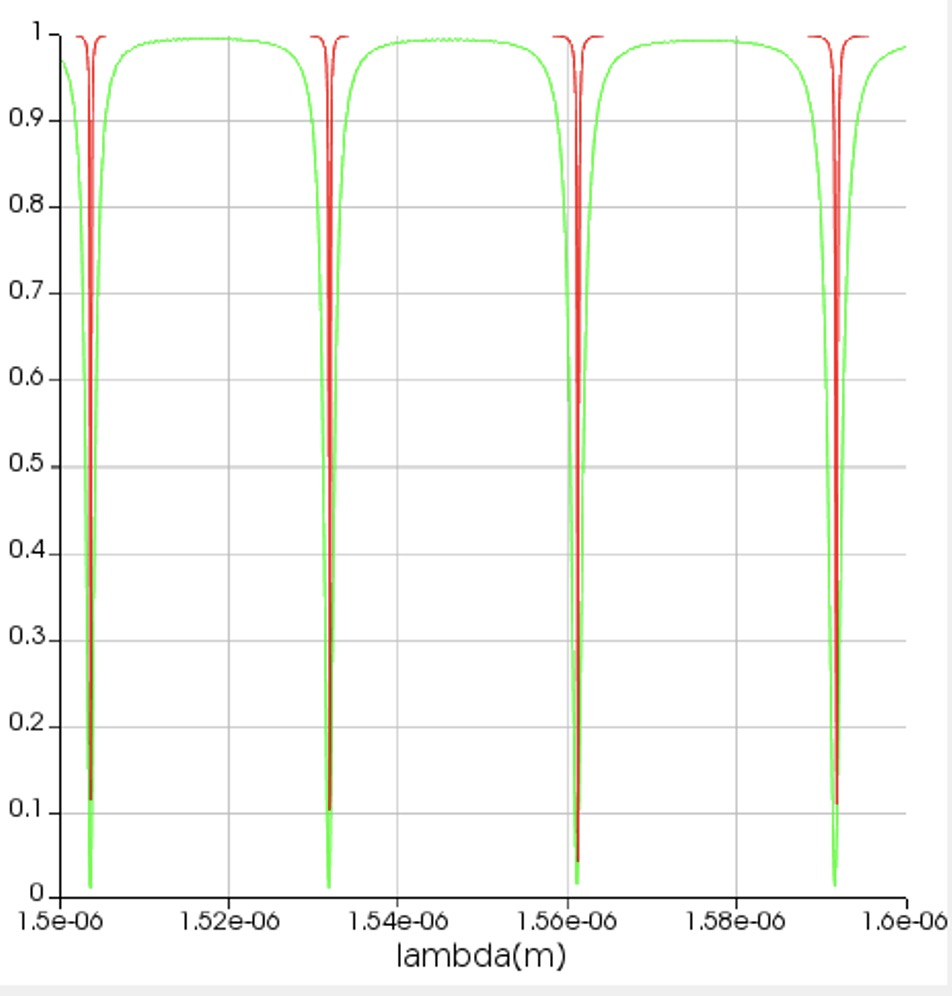
\includegraphics[width=0.45\textwidth]{img/fig3.3.png}
     \caption{Far-field radiation pattern of upward at $\Lambda=645.8\mathrm{nm}$,
     $\lambda=645.8\mathrm{nm}$ and $n_{eff}=2.4$}
     \label{fig3.3}
\end{figure}
\begin{figure}[H]
    \centering
     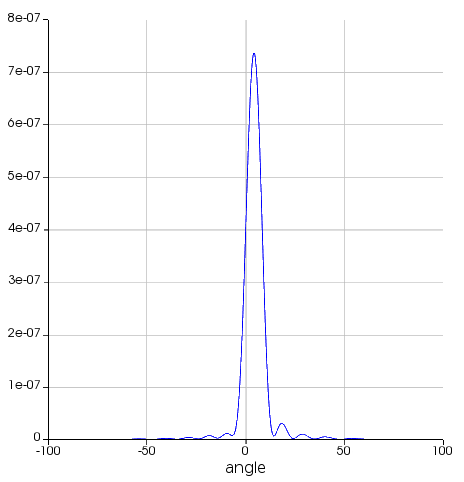
\includegraphics[width=0.45\textwidth]{img/fig3.4.png}
     \caption{Far-field radiation pattern of upward at $\Lambda=645.8\mathrm{nm}$,
     $\lambda=1468.7\mathrm{nm}$ and $n_{eff}=2.4$}
     \label{fig3.4}
\end{figure}
\begin{figure}[H]
    \centering
     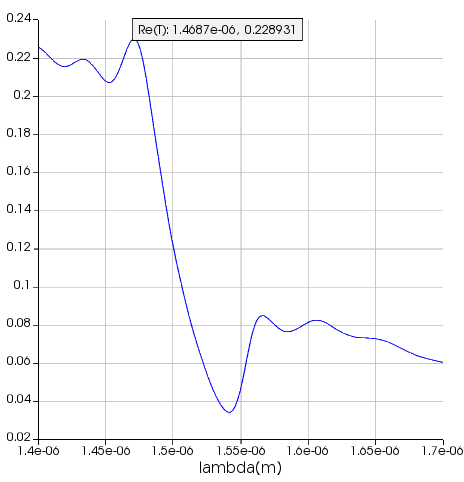
\includegraphics[width=0.45\textwidth]{img/fig3.5.png}
     \caption{The peak of upward transmission spectrum at $\Lambda=645.8\mathrm{nm}$,
     $\lambda=1468.7\mathrm{nm}$}
     \label{fig3.5}
\end{figure}
%=================================================================================================
\subsection{}
The method to correct the dip in the trasmission spectrum is 
to enlarge $\Lambda$, because the real $n_{eff}$ is smaller than the theoretical value $2.4$.
Figure \ref{fig3.6} shows that the upward transmission spectrum for $\Lambda=691.2\mathrm{nm}$, 
and the peak of transmission spectrum is $\lambda=1550.55\mathrm{nm}$. 
Figure \ref{fig3.7} illustrates the far-field radiation pattern of upward 
at $\Lambda=691.2\mathrm{nm}$ and $\lambda=1550.55\mathrm{nm}$, 
and the diffracttion angle is $3.5^\circ$, $T=6.22\times10^{-7}$.
\begin{figure}[H]
    \centering
     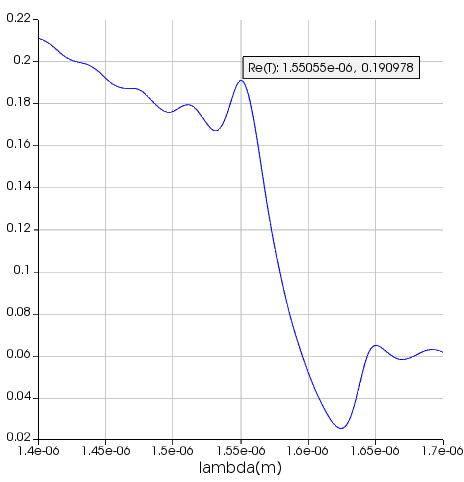
\includegraphics[width=0.45\textwidth]{img/fig3.6.png}
     \caption{Upward transmission spectrum at $\Lambda=691.2\mathrm{nm}$}
     \label{fig3.6}
\end{figure}
\begin{figure}[H]
    \centering
     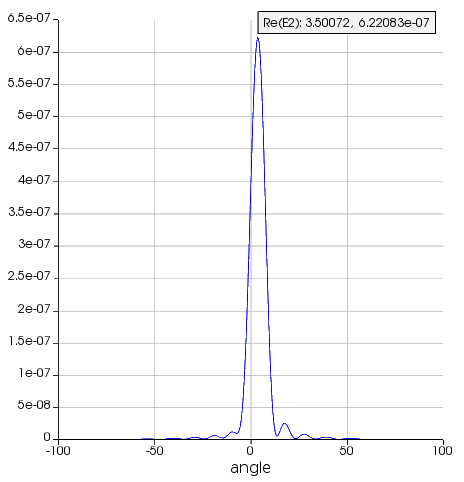
\includegraphics[width=0.45\textwidth]{img/fig3.7.png}
     \caption{Far-field radiation pattern of upward at $\Lambda=691.2\mathrm{nm}$,
     $\lambda=1550.55\mathrm{nm}$}
     \label{fig3.7}
\end{figure}
\pagebreak
%=================================================================================================

%=================================================================================================
%Appendix A
%-------------------------------------------------------------------------------------------------
% \section*{\uline{APPENDIX A}}
% %-------------------------------------------------------------------------------------------------
% Here comes some text. This text makes use of 1.5 line spacing. %=================================================================================================
% \pagebreak
%=================================================================================================
% %Appendix B
% %-------------------------------------------------------------------------------------------------
% \section*{\uline{APPENDIX B}}
% %-------------------------------------------------------------------------------------------------
% Here comes some text. This text makes use of 1.5 line spacing.\\
% In order to cite use \cite{Bern:1}, \cite{Bez:1}, \cite{BioModels}, \cite{Row:1} %=================================================================================================
% \pagebreak
% %=================================================================================================
% \bibliographystyle{plain}
% \bibliography{References}
%=================================================================================================

\end{document}